\documentclass[a4paper, openany]{memoir}

\usepackage[utf8]{inputenc}
\usepackage[T1]{fontenc} 
\usepackage[english]{babel}

\usepackage{fancyhdr}
\usepackage{float}
\usepackage{graphics}
\usepackage{amsmath}
\usepackage{amsthm}
\usepackage{amssymb}
\usepackage{enumitem}
\usepackage{multicol}
\usepackage[bookmarksopen=true,bookmarksopenlevel=2]{hyperref}
\usepackage{tikz}
\usepackage{listings}
\usepackage{xcolor}
\usepackage{indentfirst}
\usepackage{caption}
\usepackage{subcaption}

\pagestyle{fancy}
\fancyhf{}
\fancyhead[LE]{\leftmark}
\fancyhead[RO]{\rightmark}
\fancyhead[RE, LO]{Algorithmics II}
\fancyfoot[LE, RO]{\thepage}
\fancyfoot[RE, LO]{Pete Gautam}

\usetikzlibrary{positioning, automata, arrows}

\definecolor{codegreen}{rgb}{0,0.6,0}
\definecolor{codegray}{rgb}{0.5,0.5,0.5}
\definecolor{codepurple}{rgb}{0.58,0,0.82}
\definecolor{backcolour}{rgb}{0.95,0.95,0.92}

\lstdefinestyle{thestyle}{
    backgroundcolor=\color{backcolour},
    basicstyle=\ttfamily\footnotesize,
    keywordstyle=\color{red!80}\bfseries,
    ndkeywordstyle=\color{blue!80}\bfseries,
    identifierstyle=\color{black},
    commentstyle=\color{codegreen},
    stringstyle=\color{codepurple},
    breakatwhitespace=false,
    breaklines=true,
    captionpos=b,
    keepspaces=true,
    numberstyle=\tiny\color{codegray},
    numbers=left,
    numbersep=2pt,
    showspaces=false,
    showstringspaces=false,
    showtabs=false,          
    tabsize=2
}

\lstdefinelanguage{pseudocode}{ 
    keywords={new, return, this, null, if, in, while, else, for, get, set, class, and, or, not, max},
    ndkeywords={int, char, bool, void, double, true, false, Line, LineSegment, Point, Rectangle, List, Map, Edge, Graph, Queue, Vertex, Network, CNF, Clause},
    sensitive=true,
    comment=[l]{//},
    morecomment=[s]{/*}{*/},
    morestring=[b]',
    morestring=[b]"
}

\lstset{style=thestyle}

\usetikzlibrary{shapes, positioning}

\chapterstyle{thatcher}

\setcounter{chapter}{3}

\begin{document}
    \chapter{Algorithms for Hard Problems}
    In this chapter, we will look at finding algorithms for hard problems and approximations. A problem is hard is connected to it being NP-complete. In particular, we will focus on giving a feasible algorithm that solves a hard problem while allowing it to not be perfect, i.e. approximate. We will also formalise approximation algorithms and their limitations.

    A decision problem is an algorithm that returns true or false. The class $P$ is the set of decision problems that can be solved in polynomial time (with respect to the input size). The class $NP$ is the set of decision problems for which a proposed solution can be verified in polynomial time. Clearly, $P \subseteq NP$, and it is widely believed, but not proven, that $P \neq NP$.

    A decision problem $\Pi_1$ can be reduced in polynomial-time to a decision problem $\Pi_2$ if every instance of $\Pi_1$ can be converted to $\Pi_2$ with the same result. If $\Pi_1$ reduces to $\Pi_2$ and $\Pi_1 \in P$, then $\Pi_2 \in P$ as well. A problem $\Pi$ is $NP$-complete if it reduces to any other problem in $NP$ in polynomial-time. If a problem is in $P$ and $NP$-complete, then $P = NP$. Hence, if $P \neq NP$, then an $NP$-complete problem is not in $P$. We aim to find efficient algorithms to decide $NP$-complete decision problems.

    The following are some $NP$-complete problems:
    \begin{itemize}
        \item \textbf{Satisfiability (SAT)}
        \begin{itemize}
            \item Instance: a boolean expression $B$ in conjunctive normal form (CNF).
            \item Question: is $B$ satisfiable- can values be assigned to the variables to make $B$ true.
        \end{itemize}

        \item \textbf{Graph Colouring}
        \begin{itemize}
            \item Instance: a graph $G$ and a positive integer $k$.
            \item Question: can one of the $k$ colours be assigned to each vertex of $G$ so that adjacent vertices have different colours?
        \end{itemize}

        \item \textbf{Travelling Salesman Problem (TSP)}
        \begin{itemize}
            \item Instance: a complete weighted graph $G$ and a target $x$
            \item Question: is there a cycle in $G$ that visits every vertex (a `tour' of the `cities') and has total weight (length) $\leq x$?
        \end{itemize}

        \item \textbf{Hamiltonian Cycle (HC)}
        \begin{itemize}
            \item Instance: a graph $G$
            \item Question: is there a cycle in $G$ that visits every vertex exactly once?
        \end{itemize}

        \item \textbf{Vertex Cover (VC)}
        \begin{itemize}
            \item Instance: a graph $G$ and a positive integer $k$
            \item Question: is there a set $S$ of $\leq k$ vertices such that every edge has at least one endpoint in $S$?
        \end{itemize}

        \item \textbf{Clique}
        \begin{itemize}
            \item Instance: a graph $G$ and a positive integer $k$
            \item Question: is there a set $S$ of $\geq k$ vertices such that every pair of vertices of $S$ are adjacent?
        \end{itemize}

        \item \textbf{Bin Packing}
        \begin{itemize}
            \item Instance: a set $S$ of items each with positive integer size, a bin capacity $C$ and a positive integer $k$ 
            \item Question: can the items in $S$ be distributed among $\geq k$ bins so that the total size of items in each bin is $\leq C$?
        \end{itemize}

        \item \textbf{Partition}
        \begin{itemize}
            \item Instance: a collection $S$ of positive integers
            \item Question: can $S$ be partitioned into two sub-collections with equal sums?
        \end{itemize}

        \item \textbf{Longest Common Subsequence}
        \begin{itemize}
            \item Instance: a set of strings and a positive integer $k$
            \item Question: is there a string of length $\geq k$ that is a common subsequence of every string in the set?
        \end{itemize}

        \item \textbf{Shortest Common Superstring}
        \begin{itemize}
            \item Instance: a set of strings and a positive integer $k$
            \item Question: is there a string $S$ of length $\leq k$ that is a common superstring of every string in the set (i.e. a string such that every string in the set is a substring of $S$)?
        \end{itemize}

        \item \textbf{3-Dimensional Matching}
        \begin{itemize}
            \item Instance: 3 disjoint sets $X, Y, Z$ of equal size and a set $S$ of triples of the form $(x, y, z) \in X \times Y \times Z$
            \item Question: does there exist a subset of $S$ in which every element of $X, Y, Z$ appears exactly once?
        \end{itemize}

        \item \textbf{Maximum Cut}
        \begin{itemize}
            \item Instance: a weighted graph $G$ and a positive integer $k$
            \item Question: can the vertices of $G$ be split into two subsets $X$ and $Y$ such that the sum of the weights of the edges connecting $X$ to $Y$ is $\geq k$?
        \end{itemize}
    \end{itemize}

    For an $NP$-complete problem, we would like to find an efficient algorithm. It may be the case that we are only interested in solving a special kind of $NP$-complete problem that actually belongs in $P$, e.g. 2-SAT is in $P$. Another approach is to make use of a clever algorithm. Typically, the exponential-time algorithm corresponds to brute-force. So, if we have a clever algorithm that does not go through the entire solution set, we will have a more efficient algorithm even if it is exponential-time. This includes backtracking, branch-and-bound and dynamic programming. For an optimisation algorithm, we might be able to find an approximation in polynomial-time.

    \section{Backtracking}
    In this section, we will look at backtracking in detail. It is an approach that we can apply to a naive exponential-time algorithm to make it more efficient- we stop considering subsolutions that we know won't produce the result, backtrack and choose a different value for one of the chosen values. By backtracking as soon as possible, we immediately remove an infeasible solution.

    A general version of the algorithm is the following:
\begin{lstlisting}[language=pseudocode]
void choose(int i) {
    // go through all the choices
    for (x in S) {
        // add it as the next value in the solution-to-be
        a.add(i, x);
        // if a still has the potential to be a solution, 
        // move to the next value
        if (a.isOkay()) {
            // i final value in the solution => a is the solution
            if (i == n) {
                return;
            } 
            // find the next value in the solution-to-be
            else {
                choose(i+1);
            }
        }
        // at this point, choosing the value x at the i-th 
        // position does not lead to a solution, so we move
        // to the next value
        a.remove(i);
    }
}
\end{lstlisting}

    We will now look at backtracking specifically in graph colouring algorithm. The problem is to colour the vertices so that for an edge $\{u, v\}$, both the vertices $u$ and $v$ are coloured differently. The following is the algorithm for the backtracking algorithm:
\begin{lstlisting}[language=pseudocode]
// choose one of the k-colours to colour the i-th vertex
void chooseColour(int i, int k) {
    int c = 0;
    // while the graph isn't coloured and we haven't tried all the 
    // colours (for vertex i, we need not try more than i colours)
    while (!coloured && c <= min(k, i)) {
        // try colour c
        colour[i] = c;
        // if that is fine, move to the next vertex
        if (isOkay(i)) {
            if (i == numVertices) {
                coloured = true;
            } else {
                choose(i+1, k);
            }
        }
        // if that doesn't work out, move to the next colour
        c++;
    }
}

bool isOkay(int i) {
    for (int j=0; j<i-1; j++) {
        if (vertices[i].hasEdge(vertices[j]) && 
            colour[i] == colour[j]) {
            return false;
        }
    }
    return true;
}
\end{lstlisting}

    We will now illustrate the algorithm with an example. Assume that we want to colour the following graph using 2 colours.
    \begin{figure}[H]
        \centering
        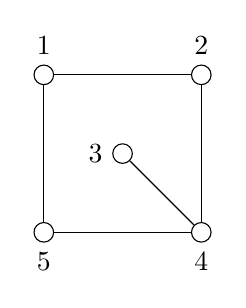
\begin{tikzpicture}
            \node[inner sep=2.5pt, circle, draw, label={90:1}] (1) at (0, 0) {};
            \node[inner sep=2.5pt, circle, draw, label={90:2}] (2) at (2, 0) {};
            \node[inner sep=2.5pt, circle, draw, label={180:3}] (3) at (1, -1) {};
            \node[inner sep=2.5pt, circle, draw, label={-90:4}] (4) at (2, -2) {};
            \node[inner sep=2.5pt, circle, draw, label={-90:5}] (5) at (0, -2) {};

            \draw (1) -- (2);
            \draw (1) -- (5);
            \draw (4) -- (2);
            \draw (4) -- (5);
            \draw (3) -- (4);
        \end{tikzpicture}
    \end{figure}
    \noindent We first colour the vertex 1 red.
    \begin{figure}[H]
        \centering
        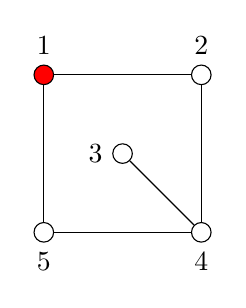
\begin{tikzpicture}
            \node[fill=red, inner sep=2.5pt, circle, draw, label={90:1}] (1) at (0, 0) {};
            \node[inner sep=2.5pt, circle, draw, label={90:2}] (2) at (2, 0) {};
            \node[inner sep=2.5pt, circle, draw, label={180:3}] (3) at (1, -1) {};
            \node[inner sep=2.5pt, circle, draw, label={-90:4}] (4) at (2, -2) {};
            \node[inner sep=2.5pt, circle, draw, label={-90:5}] (5) at (0, -2) {};

            \draw (1) -- (2);
            \draw (1) -- (5);
            \draw (4) -- (2);
            \draw (4) -- (5);
            \draw (3) -- (4);
        \end{tikzpicture}
    \end{figure}
    \noindent Since this is the first vertex, there is nothing to check. We next colour vertex 2 red.
    \begin{figure}[H]
        \centering
        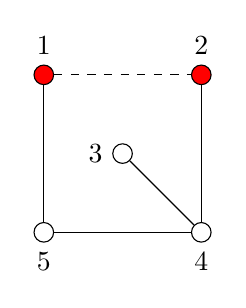
\begin{tikzpicture}
            \node[fill=red, inner sep=2.5pt, circle, draw, label={90:1}] (1) at (0, 0) {};
            \node[fill=red, inner sep=2.5pt, circle, draw, label={90:2}] (2) at (2, 0) {};
            \node[inner sep=2.5pt, circle, draw, label={180:3}] (3) at (1, -1) {};
            \node[inner sep=2.5pt, circle, draw, label={-90:4}] (4) at (2, -2) {};
            \node[inner sep=2.5pt, circle, draw, label={-90:5}] (5) at (0, -2) {};

            \draw[dashed] (1) -- (2);
            \draw (1) -- (5);
            \draw (4) -- (2);
            \draw (4) -- (5);
            \draw (3) -- (4);
        \end{tikzpicture}
    \end{figure}
    \noindent This is not a valid colouring- the vertices 1 and 2 have an edge and are both given the same colour. So, we try colouring the vertex 2 blue.
    \begin{figure}[H]
        \centering
        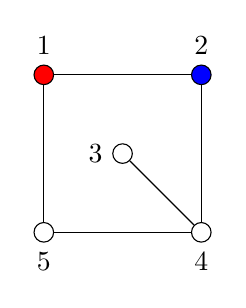
\begin{tikzpicture}
            \node[fill=red, inner sep=2.5pt, circle, draw, label={90:1}] (1) at (0, 0) {};
            \node[fill=blue, inner sep=2.5pt, circle, draw, label={90:2}] (2) at (2, 0) {};
            \node[inner sep=2.5pt, circle, draw, label={180:3}] (3) at (1, -1) {};
            \node[inner sep=2.5pt, circle, draw, label={-90:4}] (4) at (2, -2) {};
            \node[inner sep=2.5pt, circle, draw, label={-90:5}] (5) at (0, -2) {};

            \draw (1) -- (2);
            \draw (1) -- (5);
            \draw (4) -- (2);
            \draw (4) -- (5);
            \draw (3) -- (4);
        \end{tikzpicture}
    \end{figure}
    \noindent This is a valid colouring for vertices 1 and 2. We now colour vertex 3 red.
    \begin{figure}[H]
        \centering
        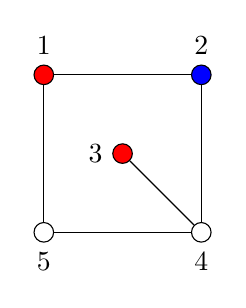
\begin{tikzpicture}
            \node[fill=red, inner sep=2.5pt, circle, draw, label={90:1}] (1) at (0, 0) {};
            \node[fill=blue, inner sep=2.5pt, circle, draw, label={90:2}] (2) at (2, 0) {};
            \node[fill=red, inner sep=2.5pt, circle, draw, label={180:3}] (3) at (1, -1) {};
            \node[inner sep=2.5pt, circle, draw, label={-90:4}] (4) at (2, -2) {};
            \node[inner sep=2.5pt, circle, draw, label={-90:5}] (5) at (0, -2) {};

            \draw (1) -- (2);
            \draw (1) -- (5);
            \draw (4) -- (2);
            \draw (4) -- (5);
            \draw (3) -- (4);
        \end{tikzpicture}
    \end{figure}
    \noindent This is a valid colouring. We next colour vertex 4 red.
    \begin{figure}[H]
        \centering
        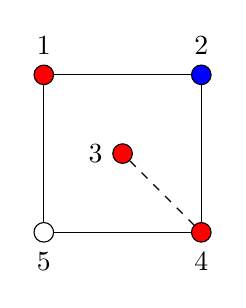
\begin{tikzpicture}
            \node[fill=red, inner sep=2.5pt, circle, draw, label={90:1}] (1) at (0, 0) {};
            \node[fill=blue, inner sep=2.5pt, circle, draw, label={90:2}] (2) at (2, 0) {};
            \node[fill=red, inner sep=2.5pt, circle, draw, label={180:3}] (3) at (1, -1) {};
            \node[fill=red, inner sep=2.5pt, circle, draw, label={-90:4}] (4) at (2, -2) {};
            \node[inner sep=2.5pt, circle, draw, label={-90:5}] (5) at (0, -2) {};

            \draw (1) -- (2);
            \draw (1) -- (5);
            \draw (4) -- (2);
            \draw (4) -- (5);
            \draw[dashed] (3) -- (4);
        \end{tikzpicture}
    \end{figure}
    \noindent This is not a valid colouring- the vertices 3 and 4 have an edge and are both given the same colour. So, we try colouring the vertex 4 blue.
    \begin{figure}[H]
        \centering
        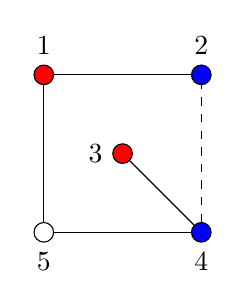
\begin{tikzpicture}
            \node[fill=red, inner sep=2.5pt, circle, draw, label={90:1}] (1) at (0, 0) {};
            \node[fill=blue, inner sep=2.5pt, circle, draw, label={90:2}] (2) at (2, 0) {};
            \node[fill=red, inner sep=2.5pt, circle, draw, label={180:3}] (3) at (1, -1) {};
            \node[fill=blue, inner sep=2.5pt, circle, draw, label={-90:4}] (4) at (2, -2) {};
            \node[inner sep=2.5pt, circle, draw, label={-90:5}] (5) at (0, -2) {};

            \draw (1) -- (2);
            \draw (1) -- (5);
            \draw[dashed] (4) -- (2);
            \draw (4) -- (5);
            \draw (3) -- (4);
        \end{tikzpicture}
    \end{figure}
    \noindent This is not a valid colouring- the vertices 2 and 4 have an edge and are both given the same colour. So, we cannot colour the vertex 4 at this point- we backtrack and colour vertex 3 blue.
    \begin{figure}[H]
        \centering
        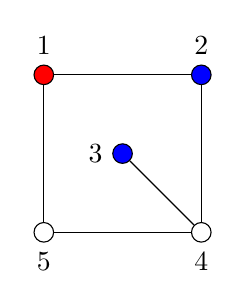
\begin{tikzpicture}
            \node[fill=red, inner sep=2.5pt, circle, draw, label={90:1}] (1) at (0, 0) {};
            \node[fill=blue, inner sep=2.5pt, circle, draw, label={90:2}] (2) at (2, 0) {};
            \node[fill=blue, inner sep=2.5pt, circle, draw, label={180:3}] (3) at (1, -1) {};
            \node[inner sep=2.5pt, circle, draw, label={-90:4}] (4) at (2, -2) {};
            \node[inner sep=2.5pt, circle, draw, label={-90:5}] (5) at (0, -2) {};

            \draw (1) -- (2);
            \draw (1) -- (5);
            \draw (4) -- (2);
            \draw (4) -- (5);
            \draw (3) -- (4);
        \end{tikzpicture}
    \end{figure}
    \noindent This is a valid colouring. So, we move to colour the vertex 4 red.
    \begin{figure}[H]
        \centering
        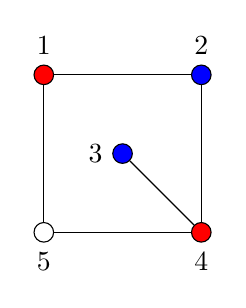
\begin{tikzpicture}
            \node[fill=red, inner sep=2.5pt, circle, draw, label={90:1}] (1) at (0, 0) {};
            \node[fill=blue, inner sep=2.5pt, circle, draw, label={90:2}] (2) at (2, 0) {};
            \node[fill=blue, inner sep=2.5pt, circle, draw, label={180:3}] (3) at (1, -1) {};
            \node[fill=red, inner sep=2.5pt, circle, draw, label={-90:4}] (4) at (2, -2) {};
            \node[inner sep=2.5pt, circle, draw, label={-90:5}] (5) at (0, -2) {};

            \draw (1) -- (2);
            \draw (1) -- (5);
            \draw (4) -- (2);
            \draw (4) -- (5);
            \draw (3) -- (4);
        \end{tikzpicture}
    \end{figure}
    \noindent This is a valid colouring. We can then try colouring vertex 5- the colour red does not work, but blue works. Hence, it is possible to colour the graph with 2 colours, with the following colouring.
    \begin{figure}[H]
        \centering
        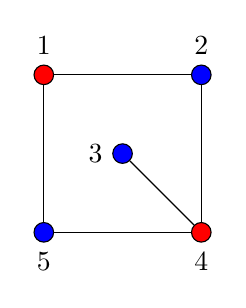
\begin{tikzpicture}
            \node[fill=red, inner sep=2.5pt, circle, draw, label={90:1}] (1) at (0, 0) {};
            \node[fill=blue, inner sep=2.5pt, circle, draw, label={90:2}] (2) at (2, 0) {};
            \node[fill=blue, inner sep=2.5pt, circle, draw, label={180:3}] (3) at (1, -1) {};
            \node[fill=red, inner sep=2.5pt, circle, draw, label={-90:4}] (4) at (2, -2) {};
            \node[fill=blue, inner sep=2.5pt, circle, draw, label={-90:5}] (5) at (0, -2) {};

            \draw (1) -- (2);
            \draw (1) -- (5);
            \draw (4) -- (2);
            \draw (4) -- (5);
            \draw (3) -- (4);
        \end{tikzpicture}
    \end{figure}

    We will now look at branch and bound for the Travelling Salesman Problem. In this problem, we are given $n$ cities and a pair of distances $d(c_i, c_j)$ for any pair of cities $c_i, c_j$. We want to compute a tour of the vertices (i.e. a path going through all the cities) that has the minimum distance. It is an optimisation problem, whose decision problem is $NP$-complete (i.e. it is $NP$-hard).

    We can use a backtracking algorithm to solve the Travelling Salesman Problem, called the branch-and-bound technique. For a solution we are producing, we produce a bound on the best possible solution it can lead to. If this is not better than those that have previously been encountered, we backtrack. There are many bounds that we can provide for the Travelling Salesman Problem, two of which are given below:
    \begin{itemize}
        \item Given a partial travelling salesman tour of length $l$, a lower bound would be
        \[l + \sum_i x_i,\]
        where the sum is over all the unvisited vertices and the value $x_i$ is the minimum distance to get from the city $c_i$ to its closest unvisited neighbour. The complete tour will involve at least travelling to the closest neighbour for a city, hence this is a valid lower bound.
        \item Given a partial travelling salesman tour of length $l$, a lower bound is $l$ added to the weight of the minimum spanning tree on the unvisited vertices, the current vertex and the starting vertex. In a travelling salesman tour, these cities must be linked by a path, which is a spanning tree. This gives a better bound in practice, but takes longer time since the minimum spanning tree must be computed for each choice at every iteration.
    \end{itemize}
    Using the lower bound, we can find out whether we can get a better length than the current one we have- if the lower bound is already greater than the best length we have found, then we can simply backtrack.
    % TODO: Complete example
    % \begin{figure}[H]
    %     \centering
    %     \begin{tikzpicture}
    %         \draw [step=0.5, opacity=0.3] (0, 0) grid (2, 3);

    %         \foreach \x in {(0, 2.5), (0.5, 1), (1.5, 0), (2, 1.5)} {
    %             \filldraw \x circle (2.5pt);
    %         }
    %     \end{tikzpicture}
    % \end{figure}

    \newpage

    \section{Pseudo-Polynomial Time Algorithms}
    In this section, we will look at a family of algorithms where the complexity depends on a number parameter. These are typically solved using dynamic programming but are not polynomial-time, as we will see.

    Consider the subset-sum (SS) problem. Given a sequence of (positive) integers $x_1, x_2$, $\dots, x_n$ and a target $t$, the problem asks whether it is possible to find a subsequence of the sequence that sums to the target $t$. For example, if we have the integers $1, 2, 4, 5$, it is possible to produce 8 by summing $5$, $2$ and $1$. It is however not possible to produce $13$ since it exceeds the sum of the given integers. It is known that the subset-sum is an $NP$-complete problem. Moreover, the partition problem is a special case of the SS problem- it fixes the target $t$ to be half the sum of the integers.

    It is possible to solve the SS problem using dynamic programming. In particular, we will keep adding numbers from the sequence of integers given and see whether it can reach the target. To determine whether the sum is equal to the target, we will also need to find out whether the sum can reach values smaller than the target- it might be possible to use this value in a later iteration to produce the target.
    
    Formally, the definition of the dynamic programming table is as follows:
    \[B[0, j] = \begin{cases}
        \texttt{true} & j = 0 \\
        \texttt{false} & \textrm{otherwise},
    \end{cases} \quad B[i, j] = B[i-1, j] \lor (x_i \leq j \land B[i-1, j-x_i]).\]
    The value $B[i, j]$ determines whether a subsequence of $x_1, x_2, \dots, x_i$ can be summed to the value $j$. At the start, we have no values in the sequence, so it is only possible to reach the target $0$. Otherwise, if the target has been reached with a subsequence of $x_1, x_2, \dots, x_{i-1}$, then it also has been reached with a subsequence of $x_1, x_2, \dots, x_i$. If this is not the case, we can ask whether $j - x_i$ could be summed to using a subsequence of $x_1, x_2, \dots, x_{i-1}$. If possible, this means that adding $x_i$ to the subsequence gives us the value $j$, i.e. it is possible to sum to $j$ using a subsequence of $x_1, x_2, \dots, x_i$. For this to be possible, we require $j - x_i$ to be positive. The answer we are looking for is $B[n, k]$.

    We will now illustrate the algorithm with an example. So, assume that we have the sequence of integers $1, 2, 4, 5$ and the target $8$. The following is the DP table for this instance of the SS problem:
    \begin{table}[H]
        \centering
        \begin{tabular}{c|ccccccccc}
            & 0 & 1 & 2 & 3 & 4 & 5 & 6 & 7 & 8 \\
            \hline
            $\varnothing$ & \texttt{T} & \texttt{F} & \texttt{F} & \texttt{F} & \texttt{F} & \texttt{F} & \texttt{F} & \texttt{F} & \texttt{F} \\
            1 &  \texttt{T} & \texttt{T} & \texttt{F} & \texttt{F} & \texttt{F} & \texttt{F} & \texttt{F} & \texttt{F} & \texttt{F} \\
            2 & \texttt{T} & \texttt{T} & \texttt{T} & \texttt{T} & \texttt{F} & \texttt{F} & \texttt{F} & \texttt{F} & \texttt{F} \\
            4 & \texttt{T} & \texttt{T} & \texttt{T} & \texttt{T} & \texttt{T} & \texttt{T} & \texttt{T} & \texttt{T} & \texttt{F} \\
            5 & \texttt{T} & \texttt{T} & \texttt{T} & \texttt{T} & \texttt{T} & \texttt{T} & \texttt{T} & \texttt{T} & {\color{red} \texttt{T}}
        \end{tabular}
    \end{table}
    \noindent Since the rightmost entry at the final row is \texttt{true}, we can reach the target 8 by a subsequence of the integers. To find the subsequence, we can traceback. In particular, from the final entry, we go up to the first \texttt{true} in the table at the same column, at which point we subtract the value given in the row and go one row above. This value is part of the subsequence. We keep doing this until we get to the top left entry. In the DP table given above, the following is its traceback:
    \begin{table}[H]
        \centering
        \begin{tabular}{c|ccccccccc}
            & 0 & 1 & 2 & 3 & 4 & 5 & 6 & 7 & 8 \\
            \hline
            $\varnothing$ & {\color{red} \texttt{T}} & \texttt{F} & \texttt{F} & \texttt{F} & \texttt{F} & \texttt{F} & \texttt{F} & \texttt{F} & \texttt{F} \\
            {\color{red} 1} &  \texttt{T} & {\color{red} \texttt{T}} & \texttt{F} & \texttt{F} & \texttt{F} & \texttt{F} & \texttt{F} & \texttt{F} & \texttt{F} \\
            {\color{red} 2} & \texttt{T} & \texttt{T} & \texttt{T} & {\color{red} \texttt{T}} & \texttt{F} & \texttt{F} & \texttt{F} & \texttt{F} & \texttt{F} \\
            4 & \texttt{T} & \texttt{T} & \texttt{T} & {\color{red} \texttt{T}} & \texttt{T} & \texttt{T} & \texttt{T} & \texttt{T} & \texttt{F} \\
            {\color{red} 5} & \texttt{T} & \texttt{T} & \texttt{T} & \texttt{T} & \texttt{T} & \texttt{T} & \texttt{T} & \texttt{T} & {\color{red} \texttt{T}}
            \end{tabular}
    \end{table}
    \noindent In this case, the bottom right entry is the first \texttt{true} value in this column. So, we subtract $5$ from the column and move to the row above. We then go one row above to find the first \texttt{true} in this column. We then subtract $2$ from the column, and then $2$ to get to the top left entry. So, the subsequence has the numbers $1, 2$ and $5$.

    The algorithm to solve the SS problem is given below:
\begin{lstlisting}[language=pseudocode]
bool subsetSum(List<int> x, int t) {
    List<List<int>> table = List.filled(x.length+1, List.filled(t+1, false));
    table[0][0] = true;

    for (int i=0; i<x.length; i++) {
        for (int j=1; j<=t; j++) {
            table[i+1][j] = table[i][j] || 
                    (x[i] <= j && table[i][j-x[i]]);
        }
    }
    return table[x.length][t];
}
\end{lstlisting}
    We will now consider the complexity of the algorithm. If we have $n$ numbers in the sequence and the target is $k$, then the algorithm runs in $O(nk)$ time. This might look like it is a polynomial-time algorithm, but it isn't. To represent the number $k$, we need $\log k$ bits. Moreover, to represent the $n$ numbers, we need $O(n \log k)$ bits (any number bigger than $k$ can be discarded since it won't be in the subsequence). Hence, the size of the input is $O(n \log k)$. If $k$ is a polynomial in $n$, then the algorithm would be a polynomial. However, the value $k$ is not bounded, e.g. if $k = 2^n$, then the input is $O(n^2)$ while the algorithm has complexity $O(n2^n)$. We refer to such algorithms as \emph{pseudo-polynomial time algorithms}; a pseudo-polynomial algorithm with input $x$ has complexity of the form $O(q(|x|, \max))$, where $q$ is a polynomial and $\max$ is the largest number in $x$. A decision problem is \emph{strongly $NP$-complete} if it admits no pseudo-polynomial time algorithm (unless $P = NP$).

    We will now look at another pseudo-polynomial time algorithm- the Knapsack problem. We are given $n$ items with weight $w_i$ and profit $p_i$, for $1 \leq i \leq n$, and a capacity $c$. We want to find the maximum profit we can get while ensuring that the total weight is below the capacity. For instance, consider the following 4 items:
    \begin{table}[H]
        \centering
        \begin{tabular}{c|cccc}
            weight & 1 & 3 & 4 & 1 \\
            \hline
            profit & 5 & 9 & 6 & 7 \\
        \end{tabular}
    \end{table}
    \noindent If the capacity is 4, then we can take items 1 and 2 to get profit 16 and weight 4.

    Before considering the pseudo-polynomial time algorithm, we will try to find a polynomial algorithm. The aim is to maximise profit and minimise weight. So, we want to prioritise the items that have a high profit-to-weight ratio. In particular, we can sort the items with respect to this value (in descending order) and then take them in order, until we meet the capacity. This doesn't work in general. For instance, the ratio for the instance we had above is the following:
    \begin{table}[H]
        \centering
        \begin{tabular}{c|cccc}
            item & 1 & 2 & 3 & 4 \\
            \hline
            weight & 1 & 1 & 3 & 4 \\
            \hline
            profit & 7 & 5 & 9 & 6  \\
            \hline
            ratio & 7 & 5 & 3 & 1.5
        \end{tabular}
    \end{table}
    \noindent So, with capacity 4, we would take the first two items- taking the next one will cross the capacity. However, this just gives a profit 12. We saw above that choosing items 1 and 3 give profit 16 and does not exceed the capacity. So, this is not a valid polynomial-time algorithm that solves the Knapsack problem. In fact, there is no polynomial-time algorithm that solves it- it is $NP$-complete.

    We will now look at the DP algorithm to solve the Knapsack problem. Like with the subset problem, we have a table where an entry $(i, j)$ lists the maximum profit we can get with item $x_i$ subject to capacity being less than $j$. So, the equation for the Knapsack problem is the following:
    \[s[0, j] = 0, \qquad s[i, j] = \begin{cases}
        s[i-1, j] & w_i > j \\
        \max(s[i-1, j], s[i-1, j-w_i] + p_i) & \text{otherwise}.
    \end{cases}\]
    When we have no items, the maximum profit we can make is always $0$. When introducing the item $x_i$, we consider whether it is more profitable to exclude the item $x_i$ (i.e. $s[i-1, j]$) or to include this item (i.e. $s[i-1, j-w_i]$ to get the best value that we can get with the other items and capacity $j-w_i$, added to the profit $p_i$ corresponding to the item $x_i$) if the weight of this item doesn't cross the capacity. The maximum profit we have is given at entry $s[n, c]$. 
    
    The pseudocode for the algorithm is given below:
\begin{lstlisting}[language=pseudocode]
int knapsack(List<int> weights, List<int> profits, int capacity) {
    List<List<int>> table = List.filled(weights.length+1, List.filled(capacity+1, 0));

    for (int i=0; i<n; i++) {
        for (int j=0; j<=capacity; j++) {
            if (weights[i] > j) {
                table[i+1][j] = table[i][j];
            } else {
                table[i+1][j] = max(table[i-1][j], 
                    table[i][j-weights[i]] + profits[i]);
            }
        }
    }

    return table[weights.length][capacity];
}
\end{lstlisting}
    The algorithm has space and time complexity $O(nc)$, making it a pseudo-polynomial time algorithm.

    We will now illustrate the algorithm with an example. Assume that we have the 4 items we had above:
    \begin{table}[H]
        \centering
        \begin{tabular}{c|cccc}
            weight & 1 & 3 & 4 & 1 \\
            \hline
            profit & 5 & 9 & 6 & 7 \\
        \end{tabular}
    \end{table}
    \noindent We will construct the dynamic programming table with capacity $4$:
    \begin{table}[H]
        \centering
        \begin{tabular}{c|ccccc}
            & 0 & 1 & 2 & 3 & 4 \\
            \hline
            $\varnothing$ & 0 & 0 & 0 & 0 & 0 \\
            $(1, 5)$ & 0 & 5 & 5 & 5 & 5 \\
            $(3, 9)$ & 0 & 5 & 5 & 9 & 14 \\
            $(4, 6)$ & 0 & 5 & 5 & 9 & 14 \\
            $(1, 7)$ & 0 & 7 & 12 & 12 & {\color{red} 16}
        \end{tabular}
    \end{table}
    \noindent So, the maximum profit we can get is 16. We can also traceback to find the items that form the optimal solution- we go to the top of the same value in the given column (from the bottom right), and then subtract the capacity by the capacity of the item, until we get to the first column. In the case above, the following is the traceback:
    \begin{table}[H]
        \centering
        \begin{tabular}{c|ccccc}
            & 0 & 1 & 2 & 3 & 4 \\
            \hline
            $\varnothing$ & 0 & 0 & 0 & 0 & 0 \\
            $(1, 5)$ & {\color{red} 0} & 5 & 5 & 5 & 5 \\
            {\color{red} $(3, 9)$} & 0 & 5 & 5 & {\color{red} 9} & 14 \\
            $(4, 6)$ & 0 & 5 & 5 & {\color{red} 9} & 14 \\
            {\color{red} $(1, 7)$} & 0 & 7 & 12 & 12 & {\color{red} 16}
        \end{tabular}
    \end{table}
    \noindent So, the second and the fourth item form part of the optimal solution, giving weight $4$ and capacity $16$.
    
    \newpage

    \section{Approximation Algorithms}
    In this section, we will look at optimisation problems where their decision problem is $NP$-complete. We will look at ways to approximate the optimal solution and see what bound we can put on the approximation to measure how good it is.

    Formally, an optimisation problem has:
    \begin{itemize}
        \item a set of instances $I$;
        \item a function \texttt{SOL}, which gives us a set of feasible solutions for an instance;
        \item a measure function $m(x, y)$ that gives every feasible solution $y$ a non-negative number with respect to an instance $x$; and
        \item a \texttt{GOAL}, which is either to find a feasible solution with maximum or minimum measure.
    \end{itemize}
    For an instance $x \in I$, we denote the optimal solution by
    \[m^*(x) = \texttt{GOAL}\{ m(x, y) \mid y \in \texttt{SOL}(x) \}.\]
    We might also want to compute the optimal solution along with the optimal measure, denoted by $y^* \in \texttt{SOL}(x)$ that satisfies $m(x, y^*) = m^*(x)$.

    We will illustrate this with an optimisation example. Consider the maximum satisfiability problem (MAX-SAT). This is an optimisation problem since it has all the 4 properties it needs to be so:
    \begin{itemize}
        \item the set of instances is the set of all boolean formulae;
        \item the set of feasible solutions for a boolean formula $B$ is the set for all (boolean) assignments for $B$;
        \item the measure function for an assignment measures how many clauses in an instance $B$ are satisfied; and
        \item the \texttt{GOAL} is to maximise.
    \end{itemize}
    For instance, consider the following CNF:
    \[(x_1 \lor \lnot x_2 \lor \lnot x_3) \land (\lnot x_1 \lor x_2 \lor x_3) \land (\lnot x_1 \lor \lnot x_2 \lor x_3).\]
    The assignment $x_1 = \texttt{false}$ and $x_2 = x_3 = \texttt{true}$ will satisfy the second and the third clause, and so has measure 2. On the other hand, setting $x_1 = x_2 = x_3 = \texttt{true} $ satisfies all the three clauses, and so has measure 3. This is the optimal solution since the boolean formula has 3 clauses.

    We can convert an optimisation problem to a decision problem. Given an optimisation problem $\Pi$, its decision version $\Pi_d$ with set of instances $I$ is given as follows: 
    \begin{itemize}
        \item \textbf{Instance}: an instance $x \in I$ and an integer $k$
        \item \textbf{Question}: is there a feasible solution $y \in \texttt{SOL}(x)$ such that $m(x, y) \leq k$ (if the goal is to minimise) or $m(x, y) \geq k$ (if the goal is to maximise)?
    \end{itemize}
    Typically, $\Pi$ is solvable in polynomial-time if and only if $\Pi_d$ is solvable in polynomial-time.

    In the specific case of MAX-SAT, its decision problem MAX-SAT-D is given below:
    \begin{itemize}
        \item \textbf{Instance}: a boolean formula $B$ and an integer $k$
        \item \textbf{Question}: does there exist a truth assignment for $B$ that satisfies at least $k$ clauses?
    \end{itemize}
    If $k = m$, where $m$ is the total number of clauses in $B$, then MAX-SAT-D is SAT, which implies that MAX-SAT-D is $NP$-complete.

    We now define the classes $NPO$ and $PO$. An optimisation problem is in $NPO$ if its decision problem is in $NP$. This includes MAX-SAT, Clique, Minimum Graph Colouring, etc. An optimisation problem is in $PO$ if its decision problem is in $P$. This includes maximum matching. We say that a problem $\Pi$ in $NPO$ is \emph{$NP$-hard} if its decision problem is $NP$-complete, e.g. MAX-SAT. We have $P = NP$ if and only if $PO = NPO$. In particular, if $P \neq NP$, then any $NP$-hard problem is not in $PO$.

    For a problem $\Pi$ in $NPO$, an \emph{exact} (or \emph{optimising}) algorithm finds an optimal solution given any instance $x$ of $\Pi$. An \emph{approximation} algorithm $A$ returns a feasible solution $A(x)$ for any instance $x$ of $\Pi$ in polynomial time. This is particular interesting if $\Pi$ is $NP$-hard. We say that an approxmiation algorithm $A$ has a \emph{performance guarantee} of $c \geq 1$ if:
    \begin{itemize}
        \item $\texttt{GOAL} = \min$ and $m(x, A(x)) \leq c \cdot m^*(x)$ for all instances $x$ of $\Pi$ or
        \item $\texttt{GOAL} = \max$ and $m(x, A(x)) \geq 1/c \cdot m^*(x)$ for all instances $x$ of $\Pi$.
    \end{itemize}
    If so, we say that $A$ is a \emph{$c$-approximation algorithm}. The closer $c$ gets to $1$, the better the approximation algorithm (and possibly the less efficient the algorithm).

    We first consider the minimum vertex cover approximation algorithm. Given a graph $G = (V, E)$, a vertex cover is a subset $U \subseteq V$ such that for any edge $e \in E$, either its source or its range is in $U$. The following is an approximation algorithm for this problem:
\begin{lstlisting}[language=pseudocode]
int approximateMinVertex(Graph g) {
    int minVertexCount = 0;
    // go through all the edges
    for (int i=0; i<g.edges.length; i++) {
        // if an edge is uncovered, add both the vertices
        if (g.edges[i].isUncovered) {
            g.cover.add(g.edges[i].source);
            g.cover.add(g.edges[i].range);
            minVertexCount += 2;
        }
    }

    return minVertexCount;
}
\end{lstlisting}
    The algorithm iterates through all the edges. If an edge is uncovered by the current vertex cover, we add both the edges that form part of this edge to the cover. Since the edge wasn't covered, we know that neither of the two vertices are part of the vertex cover, so we have added two vertices to the vertex cover.
    
    We now claim that the algorithm always gives us a vertex cover. So, let $e \in E$ be an edge. The algorithm iterates over the edge $e$ by definition. If the edge is already covered, then there is nothing to do. Otherwise, we add both the source and the range of the edge to the cover. This implies that the edge is now covered. So, we always get a vertex cover using the algorithm.

    We further claim that the algorithm has a performance guarantee of 2. That is, for a graph $G = (V, E)$ with a minimum vertex cover of size $n$, the approximation algorithm gives us at most $2n$ vertices in the vertex cover. Let $U \subseteq V$ be a vertex cover we get after executing the approximation algorithm, and let $U_o \subseteq V$ be a minimum vertex cover.
    % TODO: Complete

    We will now consider another example of approxmation algorithm, for MAX-SAT. The following is the approximation algorithm:
\begin{lstlisting}[language=pseudocode]
int approximateMAXSAT(CNF b) {
    for (int i=0; i<b.variables.length; b++) {
        b.variables[i].assign(true);
    }
    List<Clause> clauses = b.clauses;
    int satClauses = 0;

    while (clauses.isNotEmpty) {
        Variable v = clauses[0].variable[0];
        // count the number of times we have v in the clauses
        int p = clauses.countWhere(
            (clause) => clause.containsVar(v, true));
        // count the number of times we have not v in the clauses
        int q = clauses.countWhere(
            (clause) => clause.containsVar(v, false));
        
        // satisfy v or not v depending on which one 
        // is present more often in the clauses
        if (p >= q) {
            satClauses += p;
            v.assign(true);
            
            // remove satisfied clauses
            clauses.removeWhere(
                (clause) => clause.containsVar(v, true));
            
            // cannot satisfy not v => remove all such occurrences
            for (int i=0; i<clauses.length; i++) {
                clauses[i].removeVar(v, false);
            }
            
            // remove empty clauses
            clauses.removeWhere((clause) => clause.isEmpty);
        } else {
            satClauses += q;
            v.assign(false);

            clauses.removeWhere(
                (clause) => clause.containsVar(v, false));

            for (int i=0; i<clauses.length; i++) {
                clauses[i].removeVar(v, true);
            }
            
            clauses.removeWhere((clause) => clause.isEmpty);
        }
    }

    return satClauses;
}
\end{lstlisting}
    So, the algorithm works by going through all the variables and assigning them \texttt{true} or \texttt{false}, whichever assignment satisfies more clauses. We then remove the satisfied clauses and remove all occurrences of the variable from the remaining clauses (since this variable cannot lead to the clause being satisfied anymore).
    
    We now illustrate the algorithm with an example. So, assume that we have the following CNF:
    \[(x_1 \lor x_3) \land (\lnot x_1 \lor x_2) \lor (\lnot x_2 \lor \lnot x_3) \land (x_1 \lor x_2).\]
    We first assign the variable $x_2$- there are 2 occurrences of $x_2$ and one of $\lnot x_2$. So, we set $x_2 = \texttt{true}$. Then, we remove the clauses containing $x_2$ (since those have been satisfied) and the variable $\lnot x_2$ in the remaining clauses (since that value is always \texttt{false}). This gives us the following CNF:
    \[(x_1 \lor x_3) \land \lnot x_3.\]
    We now assign the variable $x_3$- there is 1 occurrence of both $x_3$ and $\lnot x_3$. So, we assign $x_3 = \texttt{true}$. This satisfies the first clause, and removing the variable $\lnot x_3$ from the second clause becomes empty. Hence, we get the assignment $x_1 = x_2 = x_3 = \texttt{true}$, which satisfies 3 of the 4 clauses. Note that the assignment $x_1 = x_2 = \texttt{true}$ and $x_3 = \texttt{false}$ satisfies all the clauses.

    We claim that the algorithm has a performance guarantee of $2$. In fact, the algorithm returns a truth assignment that satisfies at least half of the $m$ clauses, where the CNF $B$ has $m$ clauses. We prove this by inducting on the number of variables $n$ that the CNF $B$ has.
    \begin{itemize}
        \item If $n = 1$, then the possible clauses are: $x_1$, $\lnot x_1$, $(x_1 \lor \lnot x_1)$, $x_1 \land \lnot x_1$, $x_1 \land (x_1 \lor \lnot x_1)$ or $\lnot x_1 \land (x_1 \lor \lnot x_1)$. In each case, the algorithm will satisfy at least half of the clauses present.
        \item Now, assume that for some $n \geq 2$, all CNFs containing $n-1$ variables satisfies at least half of the clauses. So, let $x$ be the first variable to be assigned in the algorithm, and let $p$ be the number of clauses containing $x$, and $q$ the number of clauses containing $\lnot x$. We now break the proof into two cases, depending on the values $p$ and $q$:
        \begin{itemize}
            \item First, assume that $p \geq q$. Let $B'$ be the CNF formula resulting from deleting the clauses containing $x$ and literals $\lnot x$. It has $n-1$ variables and $r$ clauses. So, by the induction hypothesis, the algorithm has a truth assignment $f$ that satisfies at least $r/2$ clauses in $B'$. The algorithm assigns $f(x) = \texttt{true}$, so the assignment $f$ satisfies at least
            \[p + \frac{r}{2} = \frac{2p + r}{2}\]
            clauses in $B$. When constructing $B'$, we remove the $p$ clauses containing $x$ and the variable $\lnot x$ in the other $q$ clauses. So, when we remove $q$ occurrences of $\lnot x$, we remove at most $q$ clauses from $B$, i.e. $m \leq r + p + q$. Hence,
            \[\frac{2p + r}{2} \geq \frac{m + p - q}{2} \geq \frac{m}{2}\]
            since $p \geq q$. So, the result follows from induction.
            \item Now, assume that $p < q$. Let $B'$ be the CNF formula resulting from deleting the clauses containing $\lnot x$ and literals $x$. It has $n-1$ variables and $r$ clauses. So, by the induction hypothesis, the algorithm has a truth assignment $f$ that satisfies at least $r/2$ clauses in $B'$. The algorithm assigns $f(x) = \texttt{false}$, so the assignment $f$ satisfies at least
            \[q + \frac{r}{2} = \frac{2q + r}{2}\]
            clauses in $B$. When constructing $B'$, we remove the $q$ clauses containing $\lnot x$ and the variable $x$ in the other $p$ clauses. So, when we remove the $p$ occurrences of $x$, we remove at most $p$ clauses from $B$, i.e. $m \leq r + p + q$. Hence,
            \[\frac{2q + r}{2} \geq \frac{m - p + q}{2} > \frac{m}{2}\]
            since $p < q$. So, the result follows from induction.
        \end{itemize}
    \end{itemize}
    We can use this fact to show that the algorithm has a performance guarantee of $2$. Let $B$ be a boolean formula and let $k \leq m$ be the maximum number of clauses that can be satisfied in $B$. We know that the approximation algorithm gives a result satisfying 
    \[\frac{m}{2} \geq \frac{1}{2} \cdot k\]
    clauses. By definition, this implies that the algorithm has a performance guarantee of $2$. There is another approximation algorithm that has a performance guarantee of $1.2551$.

    We will look at another approximation algorithm for the TSP with triangle inequality. The triangle inequality states that for a distance function $d$ and points $x_1, x_2, x_3$, $d(x_1, x_3) \leq d(x_1, x_2) + d(x_2, x_3)$. This is true in most cases, e.g. in Euclidean geometry. The algorithm constructs a minimum spanning tree, and goes over the vertices, connecting unvisited vertices. It is called `twice-around the tree'.

    We illustrate the algorithm with an example. Consider the following set of points:
    \begin{figure}[H]
        \centering
        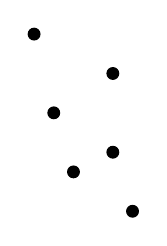
\begin{tikzpicture}
            \node[circle, draw, inner sep=1.5pt, fill=black] (a) at (0, -0.25) {};
            \node[circle, draw, inner sep=1.5pt, fill=black] (b) at (0.25, -1) {};
            \node[circle, draw, inner sep=1.5pt, fill=black] (c) at (-0.5, -0.5) {};
            \node[circle, draw, inner sep=1.5pt, fill=black] (d) at (0, 0.75) {};
            \node[circle, draw, inner sep=1.5pt, fill=black] (e) at (-0.75, 0.25) {};
            \node[circle, draw, inner sep=1.5pt, fill=black] (f) at (-1, 1.25) {};
        \end{tikzpicture}
    \end{figure}
    \noindent The minimum spanning tree for the points is given below:
    \begin{figure}[H]
        \centering
        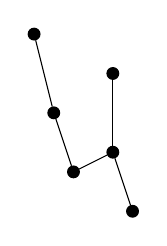
\begin{tikzpicture}
            \node[circle, draw, inner sep=1.5pt, fill=black] (a) at (0, -0.25) {};
            \node[circle, draw, inner sep=1.5pt, fill=black] (b) at (0.25, -1) {};
            \node[circle, draw, inner sep=1.5pt, fill=black] (c) at (-0.5, -0.5) {};
            \node[circle, draw, inner sep=1.5pt, fill=black] (d) at (0, 0.75) {};
            \node[circle, draw, inner sep=1.5pt, fill=black] (e) at (-0.75, 0.25) {};
            \node[circle, draw, inner sep=1.5pt, fill=black] (f) at (-1, 1.25) {};

            \draw (f) -- (e);
            \draw (e) -- (c);
            \draw (c) -- (a);
            \draw (d) -- (a);
            \draw (a) -- (b);
        \end{tikzpicture}
    \end{figure}
    \noindent We will use this to approximate the TSP. First, we replace the undirected edges with two directed edges.
    \begin{figure}[H]
        \centering
        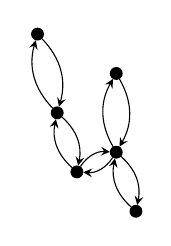
\begin{tikzpicture}
            \node[circle, draw, inner sep=1.5pt, fill=black] (a) at (0, -0.25) {};
            \node[circle, draw, inner sep=1.5pt, fill=black] (b) at (0.25, -1) {};
            \node[circle, draw, inner sep=1.5pt, fill=black] (c) at (-0.5, -0.5) {};
            \node[circle, draw, inner sep=1.5pt, fill=black] (d) at (0, 0.75) {};
            \node[circle, draw, inner sep=1.5pt, fill=black] (e) at (-0.75, 0.25) {};
            \node[circle, draw, inner sep=1.5pt, fill=black] (f) at (-1, 1.25) {};
            
            \draw[-stealth] (f) edge[bend left] (e);
            \draw[-stealth] (e) edge[bend left] (f);
            
            \draw[-stealth] (e) edge[bend left] (c);
            \draw[-stealth] (c) edge[bend left] (e);
            
            \draw[-stealth] (c) edge[bend left] (a);
            \draw[-stealth] (a) edge[bend left] (c);
            
            \draw[-stealth] (d) edge[bend left] (a);
            \draw[-stealth] (a) edge[bend left] (d);
            
            \draw[-stealth] (a) edge[bend left] (b);
            \draw[-stealth] (b) edge[bend left] (a);
        \end{tikzpicture}
    \end{figure}
    \noindent We now start from the top vertex and construct the minimum spanning tree.
    \begin{figure}[H]
        \centering
        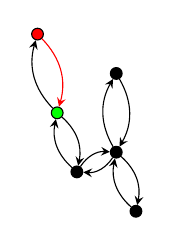
\begin{tikzpicture}
            \node[circle, draw, inner sep=1.5pt, fill=black] (a) at (0, -0.25) {};
            \node[circle, draw, inner sep=1.5pt, fill=black] (b) at (0.25, -1) {};
            \node[circle, draw, inner sep=1.5pt, fill=black] (c) at (-0.5, -0.5) {};
            \node[circle, draw, inner sep=1.5pt, fill=black] (d) at (0, 0.75) {};
            \node[circle, draw, inner sep=1.5pt, fill=green] (e) at (-0.75, 0.25) {};
            \node[circle, draw, inner sep=1.5pt, fill=red] (f) at (-1, 1.25) {};

            \draw[-stealth, red] (f) edge[bend left] (e);
            \draw[-stealth] (e) edge[bend left] (f);
            
            \draw[-stealth] (e) edge[bend left] (c);
            \draw[-stealth] (c) edge[bend left] (e);
            
            \draw[-stealth] (c) edge[bend left] (a);
            \draw[-stealth] (a) edge[bend left] (c);
            
            \draw[-stealth] (d) edge[bend left] (a);
            \draw[-stealth] (a) edge[bend left] (d);
            
            \draw[-stealth] (a) edge[bend left] (b);
            \draw[-stealth] (b) edge[bend left] (a);
        \end{tikzpicture}
    \end{figure}
    \noindent The red arrow shows directed edges in the travelling salesman tour. The visited vertices are given in red and the current vertex in green. We connect a vertex to an unvisited vertex that it is connected to, if possible. In this case, this is possible. We continue this until we get the following graph:
    \begin{figure}[H]
        \centering
        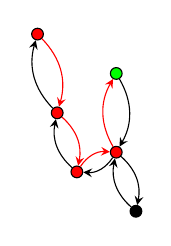
\begin{tikzpicture}
            \node[circle, draw, inner sep=1.5pt, fill=red] (a) at (0, -0.25) {};
            \node[circle, draw, inner sep=1.5pt, fill=black] (b) at (0.25, -1) {};
            \node[circle, draw, inner sep=1.5pt, fill=red] (c) at (-0.5, -0.5) {};
            \node[circle, draw, inner sep=1.5pt, fill=green] (d) at (0, 0.75) {};
            \node[circle, draw, inner sep=1.5pt, fill=red] (e) at (-0.75, 0.25) {};
            \node[circle, draw, inner sep=1.5pt, fill=red] (f) at (-1, 1.25) {};

            \draw[-stealth, red] (f) edge[bend left] (e);
            \draw[-stealth] (e) edge[bend left] (f);
            
            \draw[-stealth, red] (e) edge[bend left] (c);
            \draw[-stealth] (c) edge[bend left] (e);
            
            \draw[-stealth, red] (c) edge[bend left] (a);
            \draw[-stealth] (a) edge[bend left] (c);
            
            \draw[-stealth] (d) edge[bend left] (a);
            \draw[-stealth, red] (a) edge[bend left] (d);
            
            \draw[-stealth] (a) edge[bend left] (b);
            \draw[-stealth] (b) edge[bend left] (a);
        \end{tikzpicture}
    \end{figure}
    \noindent At this point, we must take the edge back to the visited vertex, from which we find the bottom unvisited vertex. Since we had to backtrack to find this edge, we add a shortcut from the current edge to this edge.
    \begin{figure}[H]
        \centering
        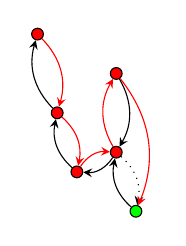
\begin{tikzpicture}
            \node[circle, draw, inner sep=1.5pt, fill=red] (a) at (0, -0.25) {};
            \node[circle, draw, inner sep=1.5pt, fill=green] (b) at (0.25, -1) {};
            \node[circle, draw, inner sep=1.5pt, fill=red] (c) at (-0.5, -0.5) {};
            \node[circle, draw, inner sep=1.5pt, fill=red] (d) at (0, 0.75) {};
            \node[circle, draw, inner sep=1.5pt, fill=red] (e) at (-0.75, 0.25) {};
            \node[circle, draw, inner sep=1.5pt, fill=red] (f) at (-1, 1.25) {};

            \draw[-stealth, red] (f) edge[bend left] (e);
            \draw[-stealth] (e) edge[bend left] (f);
            
            \draw[-stealth, red] (e) edge[bend left] (c);
            \draw[-stealth] (c) edge[bend left] (e);
            
            \draw[-stealth, red] (c) edge[bend left] (a);
            \draw[-stealth] (a) edge[bend left] (c);
            
            \draw[-stealth] (d) edge[bend left] (a);
            \draw[-stealth, red] (a) edge[bend left] (d);
            
            \draw[-stealth, dotted] (a) edge[bend left] (b);
            \draw[-stealth, red] (d) edge[bend left] (b);
            \draw[-stealth] (b) edge[bend left] (a);
        \end{tikzpicture}
    \end{figure}
    \noindent At this point, we have visited all the vertices. So, the algorithm terminates by connecting the current vertex back to the first vertex. This gives us the following tour:
    \begin{figure}[H]
        \centering
        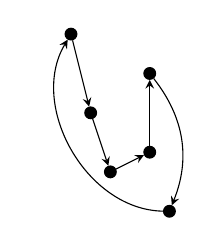
\begin{tikzpicture}
            \node[circle, draw, inner sep=1.5pt, fill=black] (a) at (0, -0.25) {};
            \node[circle, draw, inner sep=1.5pt, fill=black] (b) at (0.25, -1) {};
            \node[circle, draw, inner sep=1.5pt, fill=black] (c) at (-0.5, -0.5) {};
            \node[circle, draw, inner sep=1.5pt, fill=black] (d) at (0, 0.75) {};
            \node[circle, draw, inner sep=1.5pt, fill=black] (e) at (-0.75, 0.25) {};
            \node[circle, draw, inner sep=1.5pt, fill=black] (f) at (-1, 1.25) {};

            \draw[-stealth] (f) edge (e);
            \draw[-stealth] (e) edge (c);
            \draw[-stealth] (c) edge (a);
            \draw[-stealth] (a) edge (d);
            \draw[-stealth] (d) edge[bend left=30] (b);
            \draw[-stealth] (b) edge[bend left=60] (f);
        \end{tikzpicture}
    \end{figure}    

    For an instance $I$ of the TSP, we traverse the minimum spanning tree twice (with shortcuts). So, the distance travelled is at most $2 \cdot T$, where $T$ is the weight of the minimum spanning tree, by the triangle inequality. We also have $T \leq S$, where $S$ is the length of the shortest tour, since discarding an edge from the shortest tour gives us a spanning tree. Hence, the distance is at most $2S$, i.e. the algorithm has a performance guarantee of $2$. The Christofides' Algorithm is another approximation algorithm for TSP, with performance guarantee of $1.5$.

    The class $APX$ is composed of $NPO$ problems that admit a $c$-approximation algorithm, for some $c \geq 1$. We have seen two such problems- minimum vertex cover and MAX-SAT. We find that $PO \subseteq APX$- a problem that can be solved in polynomial time admits a $1$-approximation algorithm.

    \newpage

    \section{Approximation Schemes}
    In the previous section, we saw that some approximation algorithms for $NP$-hard problems. In the best case scenario, we should be able to find an approximation algorithm with performance guarantee as good as we want. This is what we consider in this chapter.

    Let $\Pi$ be a problem that is $NP$-hard. We say that $\Pi$ has a \emph{polynomial-time approximation scheme} (PTAS) if for every $\varepsilon > 0$, $\Pi$ has a $(1 + \varepsilon)$-approximation algorithm. Typically, we have a family of related algorithms that allows us to get an arbitrarily good approximation algorithm- we have a single algorithm with a parameter that allows us to vary the value $\varepsilon$. Each algorithm has complexity that is a polynomial time with respect to the size of the instance, but not necessarily in $1/\varepsilon$, e.g. $O(n^{1/\varepsilon})$ and $O(2^{1/\varepsilon} n^c)$. Normally, the better the approximation algorithm, the slower it is.

    We will consider a PTAS for the Subset Sum Problem. The following is the optimisation version of the problem:
    \begin{itemize}
        \item \textbf{Instance}: a sequence of positive integers $x_1, x_2, \dots, x_n$ and a number $k$.
        \item \textbf{Feasible Solutions}: a subsequence $x_{k_1}, x_{k_2}, \dots, x_{k_r}$ such that $\sum_{j=1}^r x_{k_j} \leq t$.
        \item \textbf{Measure}: $\sum_{j=1}^r x_{k_j}$.
        \item \textbf{GOAL}: $\max$.
    \end{itemize}
    So, the Subset Sum Optimisation Problem (SSO) aims to find a subsequence of $x_1, x_2, \dots, x_n$ with the highest possible sum less than the target number $k$. The problem is $NP$-hard.

    The following is the algorithm that solves the SSO problem:
\begin{lstlisting}[language=pseudocode]
int subsetSum(List<int> values, int target) {
    // keeps track of all the sums we have achieved 
    // using i integers (with respect to the for loop)
    List<int> achieved = [0];
    for (int i=0; i<values.length; i++) {
        List<int> newAchieved = achieved.map(
            (e) => e + values[i]);
        // merge the two lists achieved and newAchieved,
        // and remove those greater than target
        achieved = merge(achieved, newAchieved, target);
    }
    // return the largest value we have found
    return achieved[achieved.length-1];
}
\end{lstlisting}
    \noindent The algorithm has exponential time complexity because the list \texttt{achieved} can get arbitrarily large. To see this, fix the instance with the values list $[1, 2, 4, \dots, 2^n]$, and the target $2^{n+1}$. The algorithm iterates as follows:
    \begin{itemize}
        \item We initially have the list \texttt{achieved = [0]}.
        \item When we add the value $1$, we merge \texttt{achieved = [0]} and \texttt{newAchieved = [1]}, giving \texttt{[0, 1]}.
        \item When we add the value $2$, we merge \texttt{achieved = [0, 1]} and \texttt{newAchieved = [2, 3]}, giving \texttt{[0, 1, 2, 3]}.
        \item In general, when we add the value $2^i$, we merge \texttt{achieved = [0, 1, ..., 2\textasciicircum(i-1)]} and \texttt{newAchieved = [2\textasciicircum(i-1), 2\textasciicircum(i-1)+1, ..., 2\textasciicircum i]}, giving \texttt{[0, 1, ..., 2\textasciicircum i]}.
    \end{itemize}
    So, after the $i$-th iteration, we have the list $[0, 1, \dots, 2^i]$, which means that the \texttt{merge} function takes $2^i$ iterations. This means that the entire algorithm has complexity $O(2^n)$. 
    
    To find an approximation algorithm for SSO that runs in polynomial time, we adapt this exact algorithm. In particular, we \textit{trim} enough numbers from the list \texttt{achieved} to ensure that it has polynomial time complexity while still giving a close-to-optimal solution. First, we consider the algorithm \texttt{trim} that removes points with respect to some value $\delta$:
\begin{lstlisting}[language=pseudocode]
List<int> trim(List<int> values, double delta) {
    List<int> trimmed = [values[0]];
    int prevVal = values[0];
    for (int i=1; i<values.length; i++) {
        // if the next number is far enough from the previous 
        // number, keep it; otherwise, this number gets trimmed
        if ((1 - delta) * values[i] > prevVal) {
            trimmed.add(values[i]);
            prevVal = values[i];
        }
    }

    return trimmed;
}
\end{lstlisting}
    As we can see, the algorithm trims numbers that are quite close to a pre-existing number. For instance, if $\delta = 0.1$ and the list of values $[10, 11, 12, 15, 20, 21, 22$, $23, 24, 29]$, then:
    \begin{itemize}
        \item the trimmed list is initialised as $[10]$;
        \item the value $11$ doesn't get added since $0.9 \cdot 11 = 9.9 \leq 10$;
        \item the value $12$ gets added since $0.9 \cdot 12 = 10.8 > 10$;
        \item the value $15$ gets added since $0.9 \cdot 15 = 13.5 > 12$;
        \item the value $20$ gets added since $0.9 \cdot 20 = 18 > 15$;
        \item the value $21$ doesn't get added since $0.9 \cdot 21 = 18.9 \leq 20$;
        \item the value $22$ doesn't get added since $0.9 \cdot 22 = 19.8 \leq 20$;
        \item the value $23$ gets added since $0.9 \cdot 23 = 20.7 > 20$;
        \item the value $24$ doesn't get added since $0.9 \cdot 24 = 21.6 \leq 23$;
        \item the value $29$ gets added since $0.9 \cdot 29 = 26.1 > 24$.
    \end{itemize}
    So, we get the list $[10, 12, 15, 20, 23, 29]$. 
    
    Now, using this function, we can get a PTAS for the SSO problem, as shown below:
\begin{lstlisting}[language=pseudocode]
int subsetSumApproximation(List<int> values, int t, double delta){
    List<int> achieved = [0];
    for (int i=0; i<values.length; i++) {
        List<int> newAchieved = achieved.map(
            (e) => e + values[i]);
        // merge the two lists achieved and newAchieved, 
        // and remove those greater than t
        achieved = merge(achieved, newAchieved, t);
        // trim all the values depending on how close they are
        achieved = trim(achieved, delta);
        // return the largest value we have found
        return achieved[achieved.length-1];
    }
}
\end{lstlisting}
    It turns out if the list \texttt{values} has length $n$, then choosing the value $\delta = \frac{\varepsilon}{2n}$ gives us a $(1 + \varepsilon)$-approximation algorithm. For instance, if we want a 4-approximation algorithm, we have $\varepsilon = 3$, and $\delta = \frac{3}{2n}$. 

    The value returned by the SSO approximation algorithm is always a sum of elements in the list. Moreover, the algorithm has complexity $O(n^2 \log t/\varepsilon)$, where $t$ is the target and $n$ the length of the list. It is a polynomial in both the input size (which is $O(n \log t)$) and $\frac{1}{\varepsilon}$. Hence, this is a PTAS for the SSO problem.

    Now, the class $PTAS$ is the class of problems in $NPO$ that admit a PTAS. As we saw above, the SSO problem belongs in this class. We have $PO \subseteq PTAS$- the exact algorithm is a $(1 + \varepsilon)$-approximation algorithm for every $\varepsilon > 0$. Moreover, $PTAS \subseteq APX$, since it is composed of a specific type of approximation algorithms. If $P \neq NP$, then both the containments are strict. 

    There is a difference in the asymptotic behaviour in the two main types of $PTAS$ complexities, $O(n^{1/\varepsilon})$ and $O(n^2/\varepsilon)$. To see this, consider the following table:
    \begin{table}[H]
        \centering
        \begin{tabular}{c|cc}
            $\varepsilon$ & $O(n^{1/\varepsilon})$ & $O(n^2/\varepsilon)$ \\
            \hline
            2 & $O(n^{1/2})$ & $O(n^2/2)$ \\
            $1/2$ & $O(n^2)$ & $O(2n^2)$ \\
            $1/10$ & $O(n^{10})$ & $O(10n^2)$
        \end{tabular}
    \end{table}
    \noindent Clearly, the PTAS with complexity $O(n^2/\varepsilon)$ is more efficient than $O(n^{1/\varepsilon})$ for small values of $\varepsilon$. This is because the complexity $O(n^{1/\varepsilon})$ is exponential while $O(n^2/\varepsilon)$ is polynomial with respect to $1/\varepsilon$. With this in mind, we can define a further class- $FPTAS$ (\emph{fully polynomial time approximation schemes}), which contains polynomial time approximation schemes with complexity that is polynomial in both the input size and $1/\varepsilon$.

    \newpage

    \section{Inapproximability Results}
    In the previous two sections, we saw some approximation algorithms for $NP$-hard problems. In this section, we will show that it is not always possible to find an arbitrarily good approximation algorithm, or even one with any sort of a performance guarantee!

    For instance, consider the (Minimum) Graph Colouring Problem. The following is the optimisation problem:
    \begin{itemize}
        \item \textbf{Instance}: a graph $G = (V, E)$.
        \item \textbf{Feasible Solutions}: A colouring of $V$ such that for any edge $\{u, v\} \in E$, the vertices $u$ and $v$ are not coloured the same.
        \item \textbf{Measure}: the number of colours.
        \item \textbf{GOAL}: $\min$.
    \end{itemize}
    That is, given a graph $G$, we want to compute the fewest number of colours it takes to colour the vertices where adjacent vertices must have a different colour. It is known that the $3$-graph colouring decision problem is $NP$-complete. Hence, Minimum Graph Colouring Problem is $NP$-hard.

    We claim that Minimum Graph Colouring Problem cannot have a $c$-approxi-mation algorithm for $c < \frac{4}{3}$. Assume, for a contradiction, that there exists a $c$-approximation algorithm $A$ for the Graph Colouring Problem, with $c < \frac{4}{3}$. Now, let $G$ be a graph. If $G$ is 3-colourable, then we have $m^*(G) \leq 3$, i.e. the minimum number of colours required to colour the graph $G$ is at most $3$. So, the performance guarantee of $3/2$ implies that 
    \[m(G, A(G)) \leq c \cdot m^*(G) \leq 3c < 4.\]
    Hence, $m(G, A(G)) \leq 3$. Instead, if $G$ is not 3-colourable, then $m^*(G) \geq 4$, meaning that $m(G, A(G)) \geq 4$. That is, $m(G, A(G)) \leq 3$ if and only if $G$ is $3$-colourable. So, we can use the algorithm $A$, which by definition runs in polynomial time, to solve the 3-Colouring Decision Problem. Under the assumption that $P \neq NP$, this is a contradiction. Hence, Minimum Graph Colouring Problem does not have a $c$-approximation algorithm for $c < \frac{4}{3}$. In fact, the Minimum Graph Colouring Problem does not have a $c$-approximation algorithm for any $c \geq 1$.

    We will now look at the Bin-Packing Problem. The following is the optimisation problem:
    \begin{itemize}
        \item \textbf{Instance}: a collection $C$ of $n$ items of size $a_i$ for $1 \leq i \leq n$ and a bin capacity $n \geq 1$.
        \item \textbf{Feasible Solutions}: a partition of $C$ into some $k$ bins, where each partition has size less than $n$.
        \item \textbf{Measure}: the number of bins $k$.
        \item \textbf{GOAL}: $\min$.
    \end{itemize}
    For example, if we have items of capacity $1, 2, 3$ and bins of capacity $3$, we can fit them into 2 bins:
    \begin{figure}[H]
        \centering
        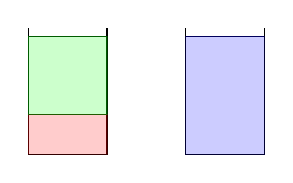
\begin{tikzpicture}
            \foreach \i in {0, 2} {
                \draw (\i, 1.6) -- (\i, 0) -- (\i+1, 0) -- (\i+1, 1.6);
            }

            \draw (0, 0.5) -- (1, 0.5);
            \draw (0, 1.5) -- (1, 1.5);
            \filldraw[red, opacity=0.2] (0, 0) rectangle (1, 0.5);
            \filldraw[green, opacity=0.2] (0, 0.5) rectangle (1, 1.5);
            
            \draw (2, 1.5) -- (3, 1.5);
            \filldraw[blue, opacity=0.2] (2, 0) rectangle (3, 1.5);
        \end{tikzpicture}
    \end{figure}

    We will use the Partition Decision Problem when showing the inapproximability of the Bin-Packing Problem. The following is the problem:
    \begin{itemize}
        \item \textbf{Instance}: a sequence of positive integers $x_1, x_2, \dots, x_n$.
        \item \textbf{Question}: can we partition the sequence into two subsequences with equal sum?
    \end{itemize}
    For example, if we have the numbers $1, 2, 3$, then we can partition them into two subsequences of equal sum: $1, 2$ and $3$.

    We claim that the Bin-Packing Problem does not have a $c$-approximation algorithm for $c < \frac{3}{2}$. Assume, for a contradiction, that there exists a $c$-approximation algorithm $A$ for the Bin-Packing Problem for $c < \frac{3}{2}$. We will use this algorithm to construct a polynomial-time algorithm for the Partition Problem. So, assume that we are given the numbers $x_1, x_2, \dots, x_n$. We will convert this instance $P$ of the Partition Problem to an instance $B$ of the Bin-Packing Problem. The capacity of the bins is 
    \[S = \frac{1}{2} \sum_{i=1}^n x_i,\]
    and we have $n$ items of size $x_1, x_2, \dots, x_n$ respectively. If the instance $P$ satisfies the Partition Problem, then it is possible to pack these items into 2 bins- both partitions must sum to $S$, so we can fit them in precisely 2 bins. Hence, $m^*(B) = 2$. Since $A$ has a performance guarantee of $c < \frac{3}{2}$, we find that
    \[m(B, A(B)) \leq c \cdot m^*(B) = c \cdot 2 < 3.\]
    Hence, $m(B, A(B)) = 2$. Instead, if $P$ does not satisfy the Partition Problem, we cannot pack the items into just 2 bins. Hence, $m^*(B) \geq 3$, meaning that $m(B, A(B)) \geq 3$. That is, $m(B, A(B)) = 2$ if and only if its corresponding instance $P$ satisfies the Partition Problem. Moreover, the algorithm runs in polynomial time- we can convert from instance $P$ to instance $B$ in constant time, and the algorithm $A$ runs in polynomial time. This gives us an algorithm that solves the Partition Problem in polynomial time. Under the assumption that $P \neq NP$, this is a contradiction. Hence, the Bin-Packing Problem does not have a $c$-approximation algorithm for $c < \frac{3}{2}$. Nonetheless, it does have a $1.5$-approximation algorithm.

    We will now look at the Travelling Salesman Problem (TSP). The following is the optimisation problem:
    \begin{itemize}
        \item \textbf{Instance}: a set $S$ of $n$ cities with a distance function $d \colon S \times S \to \mathbb{R}_{\geq 0}$.
        \item \textbf{Feasible Solutions}: a travelling salesman tour, i.e. a permutation of $1, 2, \dots, n$.
        \item \textbf{Measure}: the length of the tour.
        \item \textbf{GOAL}: $\min$.
    \end{itemize}
    We know that the TSP is $NP$-hard. To show inapproximability of the TSP, we will use the Hamiltonian Cycle Decision Problem, defined as follows:
    \begin{itemize}
        \item \textbf{Instance}: a graph $G$
        \item \textbf{Question}: Does $G$ have a cycle that visits all the vertices exactly once?
    \end{itemize}
    For instance, consider the two graphs below:
    \begin{figure}[H]
        \centering
        \begin{subfigure}[a]{0.45\textwidth}
            \centering
            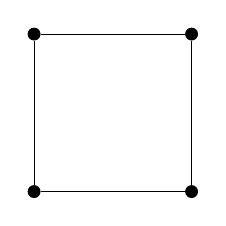
\begin{tikzpicture}
                \node[circle, draw, fill, inner sep=1.5pt] (0) at (0, 0) {};
                \node[circle, draw, fill, inner sep=1.5pt] (1) at (0, 2) {};
                \node[circle, draw, fill, inner sep=1.5pt] (2) at (2, 0) {};
                \node[circle, draw, fill, inner sep=1.5pt] (3) at (2, 2) {};

                \draw (0) -- (1);
                \draw (1) -- (3);
                \draw (3) -- (2);
                \draw (2) -- (0);
            \end{tikzpicture}
        \end{subfigure}
        \hfill
        \begin{subfigure}[a]{0.45\textwidth}
            \centering
            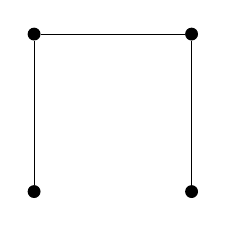
\begin{tikzpicture}
                \node[circle, draw, fill, inner sep=1.5pt] (0) at (0, 0) {};
                \node[circle, draw, fill, inner sep=1.5pt] (1) at (0, 2) {};
                \node[circle, draw, fill, inner sep=1.5pt] (2) at (2, 0) {};
                \node[circle, draw, fill, inner sep=1.5pt] (3) at (2, 2) {};

                \draw (0) -- (1);
                \draw (1) -- (3);
                \draw (3) -- (2);
            \end{tikzpicture}
        \end{subfigure}
    \end{figure}
    \noindent Then, the graph on the left has a Hamiltonian cycle while the one on the right does not.

    We shall now show that the TSP (without the triangle inequality) does not have a $c$-approximation algorithm for any $c \geq 1$. Assume, for a contradiction, that there exists a $c$-approximation algorithm $A$ for the TSP. We will use this algorithm to construct a polynomial-time algorithm for the Hamiltonian Cycle (HC) Problem. The HC problem asks whether, given a graph, there exists a cycle that visits all the vertices precisely once. So, we are given a graph $G = (V, E)$. Define the distance function $d \colon V \times V \to \mathbb{R}_{\geq 0}$ by
    \[d(u, v) = \begin{cases}
        0 & u = v \\
        1 & \{u, v\} \in E \\
        1 + nc & \textrm{otherwise},
    \end{cases}\]
    where $n = |V|$. We illustrate this with an example below- to the left, we have a graph, and to the right, we have the distances given for all pairs of distinct vertices.
    \begin{figure}[H]
        \centering
        \begin{subfigure}[a]{0.45\textwidth}
            \centering
            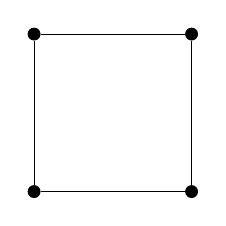
\begin{tikzpicture}
                \node[circle, draw, fill, inner sep=1.5pt] (0) at (0, 0) {};
                \node[circle, draw, fill, inner sep=1.5pt] (1) at (0, 2) {};
                \node[circle, draw, fill, inner sep=1.5pt] (2) at (2, 0) {};
                \node[circle, draw, fill, inner sep=1.5pt] (3) at (2, 2) {};

                \draw (0) -- (1);
                \draw (1) -- (3);
                \draw (3) -- (2);
                \draw (2) -- (0);
            \end{tikzpicture}
        \end{subfigure}
        \hfill
        \begin{subfigure}[a]{0.45\textwidth}
            \centering
            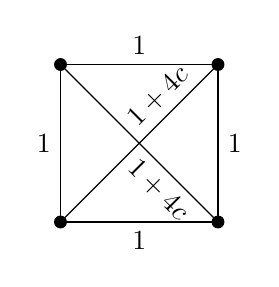
\begin{tikzpicture}
                \node[circle, draw, fill, inner sep=1.5pt] (0) at (0, 0) {};
                \node[circle, draw, fill, inner sep=1.5pt] (1) at (0, 2) {};
                \node[circle, draw, fill, inner sep=1.5pt] (2) at (2, 0) {};
                \node[circle, draw, fill, inner sep=1.5pt] (3) at (2, 2) {};

                \draw (0) -- node[left] {1} (1);
                \draw (1) -- node[above] {1} (3);
                \draw (3) -- node[right] {1} (2);
                \draw (2) -- node[below] {1} (0);
                \draw (0) -- node[above right, rotate=45] {$1 + 4c$} (3);
                \draw (1) -- node[below right, rotate=-45] {$1 + 4c$} (2);
            \end{tikzpicture}
        \end{subfigure}
    \end{figure}
    \noindent We can see that if the graph $G$ has a HC, then we can find a Travelling Salesman tour of length $n$, i.e. $m^*(G) = n$. Since $A$ has a performance guarantee of $c$, we find that $m(G, A(G)) \leq nc$. Now, if $G$ does not have a HC, then the the Travelling Salesman tour must take one of the edges not in $E$. To see this, consider the following example graph.
    \begin{figure}[H]
        \centering
        \begin{subfigure}[a]{0.45\textwidth}
            \centering
            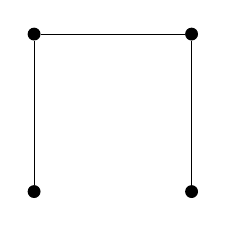
\begin{tikzpicture}
                \node[circle, draw, fill, inner sep=1.5pt] (0) at (0, 0) {};
                \node[circle, draw, fill, inner sep=1.5pt] (1) at (0, 2) {};
                \node[circle, draw, fill, inner sep=1.5pt] (2) at (2, 0) {};
                \node[circle, draw, fill, inner sep=1.5pt] (3) at (2, 2) {};

                \draw (0) -- (1);
                \draw (1) -- (3);
                \draw (3) -- (2);
            \end{tikzpicture}
        \end{subfigure}
        \hfill
        \begin{subfigure}[a]{0.45\textwidth}
            \centering
            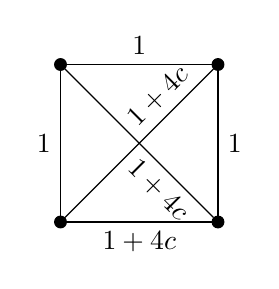
\begin{tikzpicture}
                \node[circle, draw, fill, inner sep=1.5pt] (0) at (0, 0) {};
                \node[circle, draw, fill, inner sep=1.5pt] (1) at (0, 2) {};
                \node[circle, draw, fill, inner sep=1.5pt] (2) at (2, 0) {};
                \node[circle, draw, fill, inner sep=1.5pt] (3) at (2, 2) {};

                \draw (0) -- node[left] {1} (1);
                \draw (1) -- node[above] {1} (3);
                \draw (3) -- node[right] {1} (2);
                \draw (2) -- node[below] {$1 + 4c$} (0);
                \draw (0) -- node[above right, rotate=45] {$1 + 4c$} (3);
                \draw (1) -- node[below right, rotate=-45] {$1 + 4c$} (2);
            \end{tikzpicture}
        \end{subfigure}
    \end{figure}
    \noindent Clearly, it does not have a Travelling Salesman Tour of length $n$. Moreover, there are at least $n-1$ other edges we take, and each edge has length $\geq 1$. Hence,
    \[m(G, A(G)) \geq (1 + nc) + (n - 1) = nc + n > nc.\]
    This implies that $m(G, A(G)) \leq nc$ if and only if $G$ has a HC. This gives us a polynomial-time algorithm to solve the HC problem, which leads to a contradiction. So, TSP cannot have a $c$-approximation algorithm.

\end{document}